\section{eo\-File\-Snapshot Class Reference}
\label{classeo_file_snapshot}\index{eoFileSnapshot@{eoFileSnapshot}}
Prints snapshots of fitnesses to a (new) file every N generations.  


{\tt \#include $<$eo\-File\-Snapshot.h$>$}

Inheritance diagram for eo\-File\-Snapshot::\begin{figure}[H]
\begin{center}
\leavevmode
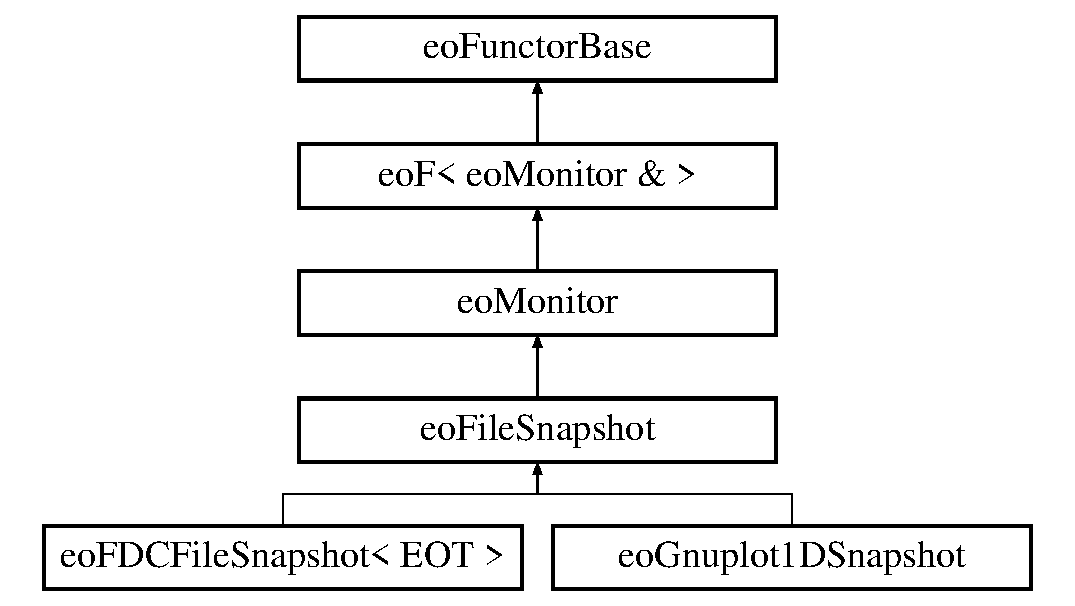
\includegraphics[height=5cm]{classeo_file_snapshot}
\end{center}
\end{figure}
\subsection*{Public Types}
\begin{CompactItemize}
\item 
typedef std::vector$<$ double $>$ {\bf v\-Double}\label{classeo_file_snapshot_w0}

\item 
typedef {\bf eo\-Value\-Param}$<$ std::vector$<$ double $>$ $>$ {\bf v\-Double\-Param}\label{classeo_file_snapshot_w1}

\end{CompactItemize}
\subsection*{Public Member Functions}
\begin{CompactItemize}
\item 
{\bf eo\-File\-Snapshot} (std::string \_\-dirname, unsigned \_\-frequency=1, std::string \_\-filename=\char`\"{}gen\char`\"{}, std::string \_\-delim=\char`\"{} \char`\"{}, unsigned \_\-counter=0, bool \_\-rm\-Files=true)\label{classeo_file_snapshot_a0}

\item 
virtual bool {\bf has\-Changed} ()\label{classeo_file_snapshot_a1}

\begin{CompactList}\small\item\em accessor: has something changed (for gnuplot subclass) \item\end{CompactList}\item 
unsigned {\bf get\-Counter} ()\label{classeo_file_snapshot_a2}

\begin{CompactList}\small\item\em accessor to the counter: needed by the gnuplot subclass \item\end{CompactList}\item 
std::string {\bf get\-File\-Name} ()\label{classeo_file_snapshot_a3}

\begin{CompactList}\small\item\em accessor to the current filename: needed by the gnuplot subclass \item\end{CompactList}\item 
void {\bf set\-Current\-File\-Name} ()\label{classeo_file_snapshot_a4}

\begin{CompactList}\small\item\em sets the current filename depending on the counter \item\end{CompactList}\item 
{\bf eo\-Monitor} \& {\bf operator()} (void)\label{classeo_file_snapshot_a5}

\begin{CompactList}\small\item\em The operator(void): opens the std::ostream and calls the write method. \item\end{CompactList}\item 
{\bf eo\-Monitor} \& {\bf operator()} (std::ostream \&\_\-os)\label{classeo_file_snapshot_a6}

\begin{CompactList}\small\item\em The operator(): write on an std::ostream. \item\end{CompactList}\item 
virtual const std::string {\bf get\-Dir\-Name} ()\label{classeo_file_snapshot_a7}

\item 
virtual const std::string {\bf base\-File\-Name} ()\label{classeo_file_snapshot_a8}

\item 
void {\bf add} (const {\bf eo\-Param} \&\_\-param)\label{classeo_file_snapshot_a9}

\begin{CompactList}\small\item\em add checks whether it is a std::vector of doubles \item\end{CompactList}\end{CompactItemize}
\subsection*{Private Attributes}
\begin{CompactItemize}
\item 
std::string {\bf dirname}\label{classeo_file_snapshot_r0}

\item 
unsigned {\bf frequency}\label{classeo_file_snapshot_r1}

\item 
std::string {\bf filename}\label{classeo_file_snapshot_r2}

\item 
std::string {\bf delim}\label{classeo_file_snapshot_r3}

\item 
unsigned int {\bf counter}\label{classeo_file_snapshot_r4}

\item 
std::string {\bf current\-File\-Name}\label{classeo_file_snapshot_r5}

\item 
bool {\bf bool\-Changed}\label{classeo_file_snapshot_r6}

\end{CompactItemize}


\subsection{Detailed Description}
Prints snapshots of fitnesses to a (new) file every N generations. 

Assumes that the parameters that are passed to the monitor (method add in {\bf eo\-Monitor.h}{\rm (p.\,\pageref{eo_monitor_8h})}) are {\bf eo\-Value\-Param}{\rm (p.\,\pageref{classeo_value_param})}$<$std::vector$<$double$>$ $>$ of same size.

A dir is created and one file per snapshot is created there - so you can later generate a movie!

TODO: The counter is handled internally, but this should be changed so that you can pass e.g. an evalcounter (minor)

I failed to templatize everything so that it can handle {\bf eo\-Param}{\rm (p.\,\pageref{classeo_param})}$<$std::vector$<$T$>$ $>$ for any type T, simply calling their get\-Value method ... 



Definition at line 53 of file eo\-File\-Snapshot.h.

The documentation for this class was generated from the following file:\begin{CompactItemize}
\item 
eo\-File\-Snapshot.h\end{CompactItemize}
